% ---------------------------------------------------------------------
\section{Sampling: from a prohibition to a coverage condition}

\Q What must a sampling schedule do? The rule should be stated so that a protocol writer who
obeys it literally cannot still defeat it.

\D The rule was restated as the lap condition $n\varepsilon \ge T$ for a step
$h = T + \varepsilon$. Partial laps were priced at fixed $n$, and a search was made for a
schedule that avoids every multiple of $T$ and still fails (\texttt{\rn{gen.lattice}}).
Figure 6 was redrawn as a phase overlay that separates the phases a schedule reaches from
the phases its step makes available (\texttt{\rn{gen.phaseclock}}). This text reached main
on \rn{git.main_lap}.

\F The prohibition was necessary but not sufficient.
\begin{itemize}
\item \textbf{The condition.} The requirement is $\varepsilon \ge T/n$. Over
\rn{new.lap_horizon_y} years, $n = \rn{new.lap_n}$ fortnightly visits, so
$\varepsilon \ge \rn{new.lap_eps_h}$~h.
\item \textbf{It is a threshold, not a cliff.} The table gives sd$(\ln\hat\theta)$ against a
schedule that laps, at the same $n$:
\begin{center}\small
\begin{tabular}{lccccc}
\toprule
fraction of a lap swept & $\rn{lnew.lapfrac_a}\%$ & $\rn{lnew.lapfrac_b}\%$ & $\rn{lnew.lapfrac_c}\%$
 & $\rn{lnew.lapfrac_d}\%$ & $\rn{lnew.lapfrac_e}\%$ \\
cost & $\rn{new.lap_cost_04}\times$ & $\rn{new.lap_cost_10}\times$ & $\rn{new.lap_cost_25}\times$
 & $\rn{new.lap_cost_50}\times$ & $\rn{new.lap_cost_75}\times$ \\
\bottomrule
\end{tabular}
\end{center}
\item \textbf{The counterexample.} A step of $\rn{new.near_step}$~d avoids every multiple of
$T$ and reaches $\rn{new.near_phases}$ distinct phases, more than any other schedule. But
those phases are packed into $\rn{new.near_span_h}$~h of the dial, and
sd$(\ln\hat\theta) = \rn{new.near_sd}$, against $\rn{new.sd_monthly}$ for the monthly design.
\item \textbf{A few hours on the step buy back the lost visits.} At $\rn{lnew.n20_n}$ visits a
lap needs $\varepsilon \ge \rn{new.lap_eps_h_n20}$~h. Booking every
$\rn{new.lap_step_n20}$~d instead of every $\rn{lnew.step_off_v}$~d takes sd from
$\rn{new.sd_n20_off}$ to $\rn{new.sd_n20_lap}$.
\item \textbf{Phases reached, out of phases available.} Monthly: $\rn{new.reached_monthly}$
of $\rn{new.available_monthly}$. Every $\rn{lnew.step_off_v}$~d: $\rn{new.reached_off}$ of
$\rn{new.available_off}$. Every $\rn{calc.T}$~d: $\rn{new.reached_fortnightly}$ of
$\rn{new.available_fortnightly}$. A bare phase count only reports the visit count back; the
lattice of available phases binds only on the fortnightly step.
\end{itemize}

\begin{figure}[htbp]
\centering
\begin{minipage}[b]{0.515\textwidth}\centering
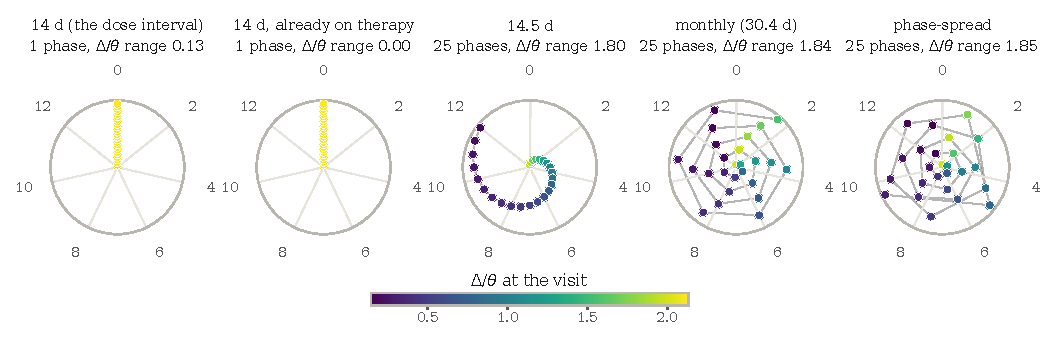
\includegraphics[width=\linewidth]{phaseclock_0920}\\[-1pt]
{\footnotesize (a) 20 Sept: polar dial, one spoke at the dose interval}
\end{minipage}\hfill
\begin{minipage}[b]{0.465\textwidth}\centering
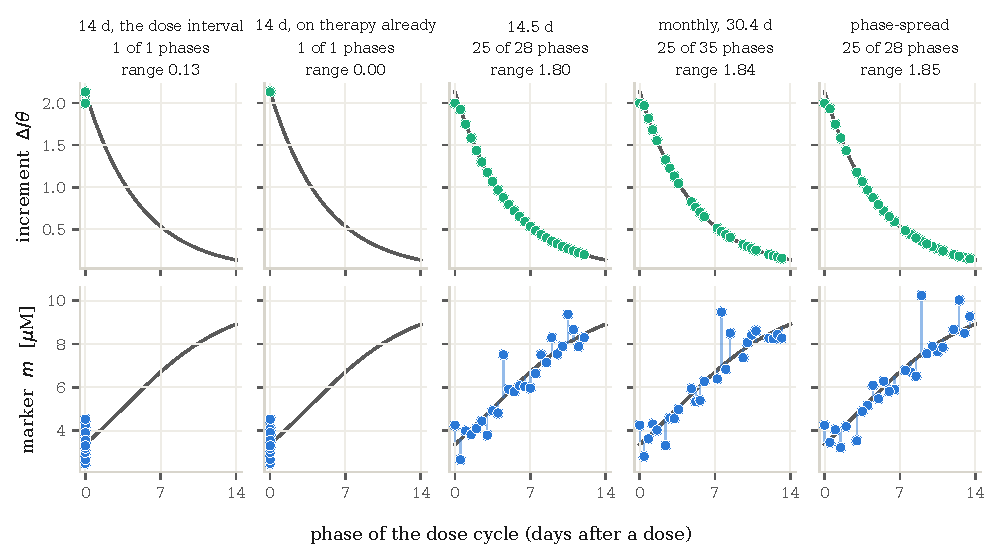
\includegraphics[width=\linewidth]{phaseclock_0927}\\[-1pt]
{\footnotesize (b) 27 Sept: increment and marker folded onto the cycle}
\end{minipage}
\caption{Figure 6 of the paper (§4.3) as it stood in each draft. Both drafts load the same
file, \texttt{results/figures/fig\_E1\_phaseclock.pdf}. That file was overwritten
\rn{git.fig6_commits} times after 20 Sept, first in \texttt{\rn{git.fig6_first}}
(\rn{git.fig6_first_date}). Each panel here is therefore regenerated by its own draft's
\texttt{audit/g1\_phase\_clock.py}, run in a temporary worktree by \texttt{fig\_phaseclock.py}.
Panel (b) shows why a phase count is not coverage. The $\rn{lnew.step_off_v}$~d schedule
reaches $\rn{new.reached_off}$ of $\rn{new.available_off}$ phases, yet over these draws it
spans only $\rn{new.range_off}$ of $\Delta/\theta$, against $\rn{new.delta_range_off}$ once
its lap is complete.}
\label{fig:clock}
\end{figure}

\W
\begin{center}\small
\begin{tabularx}{\textwidth}{@{}p{2.7cm}LL@{}}
\toprule
 & \textbf{20 Sept} & \textbf{27 Sept} \\
\midrule
Remark 4, §4.1 & ``\rn{lold.remark4_title}''; aliasing cost $\rn{old.alias_cost}\times$
 & ``\rn{lnew.remark4_title}''; lap inequality, partial-lap table, the
 $\rn{new.near_step}$~d counterexample, the $\rn{lnew.n20_n}$-visit result; aliasing cost
 unchanged at $\rn{new.alias_cost}\times$ \\
Figure 6, §4.3 & polar dial, radius $=$ visit order, one spoke at $\rn{calc.T}$~d
 & two rows (increment, marker), with headers giving phases reached of phases available \\
Tier 3, §6.4 & ``one hard exclusion'': do not sample on dosing days & ``one hard
 requirement'': complete one lap; the gap in ``avoid multiples'' is stated \\
generated numbers & no lattice or phase-clock keys & \texttt{lattice.tex} and
 \texttt{phaseclock.tex}, both new \\
\bottomrule
\end{tabularx}
\end{center}

\Out{The protocol rule is ``complete one lap of the dose cycle''. ``Avoid multiples of the
dose interval'' is necessary but not sufficient.}
